\section{\label{ManipulatorModel}マニピュレータ}
\markright{\arabic{section}. マニピュレータ}
\hfill {\em documented by Hiromu Onda}

{\bf rotational-joint}クラスと{\bf manipulator}クラスのインスタンスからマニピュレータ
モデルは構成される。{\bf rotational-join}クラスは、{\bf body}のサブクラスであり、
マニピュレータの間接モデルを定義する。
{\bf manipulator}は、{\bf cascaded-coords}のサブクラスであり、運動方程式と逆運動方程式の
解を求めるメソッドを持っている。

マニピュレータを定義するには、
すべての関節を作成した後、{\bf manipulator}にそれらを統合する。

\subsection{
%\label{JointModel}
関節のモデル}

クラス{\bf rotational-joint}が関節のモデルを記述する。
クラス{\bf rotational-joint}は、{\bf body}をスーパクラスに持ち、
その形状モデル、座標系に加えて
関節回転軸、回転角度、可動角度範囲、などを管理している。
次の{\bf defjoint}マクロによって{\bf rotational-joint}
のインスタンスが作成され、{\em joint-name}にバインドされる。
{\bf parent}には、親の関節を指定する。
ベースと指には可動軸を指定する必要はない。

\begin{refdesc}
\longdescription{defjoint}{joint-name \&key \= :shape \hspace{10mm}\= {\it body-object} \` [マクロ]\\
% \hspace{70mm} [マクロ]\\
\> :color \> {\it color-id} \hspace{2cm} \= ;0-15 for MMD \\
\> :parent \> {\it parent-joint} \\
\> :axis \> {\it rotational-axis} \>  ; :x, :y or :z \\
\> :offset \> {\it trans-from-parent-joint} \\
\> :low-limit \> {\it joint-angle-limit-low} \\
\> :high-limit \> {\it joint-angle-limit-hight}}{
関節のモデルを記述する。}
\end{refdesc}

\subsection{
%\label{MultiJointsManipulator}
多関節マニピュレータ}

マニピュレータモデルはクラス{\bf manipulator}によって記述される。
マニピュレータモデルを作成するには、
次の{\bf defmanipulator}マクロを用いる。

\begin{refdesc}
\longdescription{defmanipulator}{manipulator-name \&key \= :class \hspace{2cm} \= {\it manipulator-class} \` [マクロ]\\
%manipulator-class} \hspace{25mm} [マクロ]\\
\> :base \> {\it base-joint} \\
\> :joints \>  {\it list-of-all-joints} \\
\> :hand \> {\it handjoint} \\
\> :left-finger \> {\it left-finger}\\
\> :right-finger \> {\it right-finger}\\
\> :handcoords \> {\it trans-from-hand-to-armsolcoords}\\
\> :toolcoords \> {\it trans-from-armsolcoords-to-toolcoords} \\
\> :open-direction \> {\it finger-open-direction}\\
\> :right-handed  \> {\it righty-or-lefty}}{
マニピュレータモデルを作成する。}

\classdesc{rotational-joint}{body}{(axis offset high-limit low-limit)}
{6自由度マニピュレータの間接を記述する。}

\classdesc{manipulator}{cascaded-coords}{(base baseinverse joint angles right-handed hand handcoords\\
\> right-finger left-finger openvec max-span\\
\> toolcoords toolinverse armsolcoords toolinverse armsocoords\\
\> approach grasp affix)}
{ベースからハンドまでのマニピュレータの運動を管理する。}

\methoddesc{:newcoords}{newrot \&optional newpos}{ 
関節角度が限度に収まっていれば座標系を
{\em newrot}と{\em newpos}に更新する 
}
\methoddesc{:armsolcoords }{}{
ベース座標系からハンド座標系への変換(座標系のインスタンス)を計算し、作成する。
%  ベースからハンドに至る変換を求める
}
\methoddesc{:tool}{\&rest msg}{
 工具座標系を返す、または変更する
}
\methoddesc{:set-tool}{newtool \&optional offset copy}{
 工具座標系{\tt toolcoords}に{\em newtool}を設定する
}
\methoddesc{:reset-tool }{}{
 工具座標系を初期値に戻す
}
\methoddesc{:worldcoords }{}{
 工具座標系の位置ベクトル、回転行列、座標系のワールド表現を求める
}
\methoddesc{:set-coords }{}{
順運動の解を求めるために、座標系を強制的に設定する。
% 一旦順キネマを計算し、そこからさらに各関節角度を求める
}
\methoddesc{:config }{\&optional (a newangles)}{
 6つの関節角度を直接に設定する
}
\methoddesc{:park }{}{
 初期姿勢に戻す
}
\methoddesc{:hand}{\&optional (h nil)}{
 ハンドオブジェクトを返す
}
\methoddesc{:handcoords}{}{
 ハンド座標系の位置ベクトル、回転行列、座標系のワールド表現を求める
}
\methoddesc{:span}{}{
 現在の指の間隔を返す
}
\methoddesc{:open-fingers}{s \&optional abs \&aux (current (send self :span))}
{
 指幅を相対的、絶対的に指定する
}
\methoddesc{:close-fingers}{}{
 指を完全に閉じる 
}
\methoddesc{:angles}{\&optional flag}{
 現在の姿勢の関節角度のリストを返す
}

% \methoddesc{:right-handed}{}{
%% ソースそのものがありませんでした。
% 右手姿勢、左手姿勢を選択する
%}

\methoddesc{:get-approach }{}{
 現在アプローチしている対象を返す
}
\methoddesc{:set-approach }{a}{
 アプローチ対象{\it a}を設定する
}
%\methoddesc{:get-grasp}{}{
%(:get-grasp () grasp-config)
%??? 
% 把握姿勢にある対象物を返す
%}
\methoddesc{:set-grasp}{g}{
 把握対象物{\it g}を指定する
}
\methoddesc{:get-affix}{}{
 把握している物体を返す
}
\methoddesc{:affix}{\&optional (grasp)}{
{\bf affixed-object}に{\tt grasp}を設定する。
{\tt grasp}は、子孫として{\tt handcoords}に関連付けられる。
% 把握を指示する
}
\methoddesc{:unfix}{\&optional (margin 10.0)}{
{\bf affixed-object}にNILを設定する。
{\tt grasp}は、{\tt handcoords}の子孫リストから外される。
% 把握物体を解放したことを指示する
}
\longdescription{:create}{\= \&rest args \` [メソッド]\\
%\longdescription{:create}{\= \&rest args \hspace{111mm} [メソッド]\\
\> \&key \= (:name nm) (:hand h) (:joints j)\\
\> \> (:left-finger lf) (:right-finger rf)\\
\> \> ((:toolcoords tc) (make-coords))\\
\> \> ((:handcoords hc) (make-coords))\\
\> \> ((:base bs) (make-cascoords))\\
\> \> (open-direction (floatvector 0 1 0))\\
\> \> ((:max-span mspan) 100.0)\\
\> \> ((:lefty lft) t)\\
\> \> ((:act a) nil)\\
\> \&allow-other-keys}{
新しいマニピュレータオブジェクトを作成、初期化する
}
\end{refdesc}

{\bf manipulator}オブジェクトは、
{\bf base、joints(J1\ldots J6)、handcoords、toolcoords}
の座標系の繋がりを管理する。
%図\ref{ManipulatorObject}に{\bf manipulator}オブジェクトのスロット構成を、
%表\ref{ManipulatorMethods}に受け付けられるメソッドを掲げる。
{\bf manipulator}クラスは、{\bf cascaded-coords}のサブクラスであり、
やはり、{\bf cascaded-coords}(または{\bf body}などのサブクラス)
である{\bf base}に結合され、
{\bf base}から{\bf toolcoords}(手先座標系)への変換を管理している。
したがって、{\bf manipulator}オブジェクトに対して送られる
{\bf :translate、:locate、:rotate、:orient、:transform}
などのメッセージは、手先点に対して作用する。
そのとき同時にWRTパラメータを指定すれば、
手先はWRT座標系に対して動く。
次のプログラムでは、{\bf eta3}を{\bf manipulator}のインスタンスと仮定している。

\begin{verbatim}
 (send eta3 :translate #f(0 0 -100))        ;手先を10cm引っ込める 
 (send eta3 :translate #f(0 0 -100) :world) ;10cm下げる
 (send eta3 :translate #f(0 0 -100)
             (manipulator-base eta3))     ;手先をベース座標系で10cm下げる
\end{verbatim}

これらのメッセージに対して、manipulatorはアーム解を計算して6つの
関節角度を決定する。
一般に解は複数存在するが、{\bf right-handed}(右手系、左手系)
の区別、および現在の関節角度との連続性により適当な解が選択される。
しかし、指定された位置、姿勢に対する解が存在しない場合や関節角が
限界を越える場合は移動、回転は起こらず、警告が発せられる。

アーム解の計算は、実際のマニピュレータに対応した
個々のmanipulatorクラスに定義された{\bf :armsol}メソッドが行う。
マニピュレータがワールド座標系のどこに置かれてもよいように、
また、どのような工具を用いてもよいように、アーム解は、
{\bf base、toolcoords}とは独立に、base座標系中でのハンドの位置、姿勢に
対して与えられる。

{\bf base、J1、J2、\ldots 、handcoords、toolcoords}の関係を図\ref{JointCoords}
に示す。
ワールドから手先への変換を$T$とすると、$T$および各部分変換は次のようにし
て得られる。

$
\begin{array}{ll}
T & = base \cdot J1 \cdot J2 \cdot \ldots 
\cdot J6 \cdot handcoords \cdot toolcoords \\ 
 & = (send \; eta3 \; :worldcoords) \\ 
T_{Jn} & = base \cdot J1\cdot \ldots \cdot Jn \\
 & = (send \; Jn \; :worldcoords) \\
T_{arm} & = J1 \cdot J2 \cdot \ldots \cdot J6 \cdot handcoords \\ 
 & = (send \; eta3 \; :armsol-coords) \\ 
T_{tool} & = J1 \cdot J2 \cdot  \ldots \cdot J6 \cdot handcoords \cdot toolcoords \\ 
 & = (send \; eta3 \; :copy-coords) \\
T_{t} & = toolcoords \\ 
 & = (manipulator-toolcoords \; eta3)\\
T_{t}^{-1} & = toolcoords^{-1} \\ 
 & = (manipulator-toolinverse \; eta3) \\
T_{h} & = handcoords \\ 
 & = (manipulator-handcoords \; eta3)\\
\end{array}$

ここで、$T$はワールド座標系から工具座標系まで変換する。

\begin{figure}
\begin{center}
%%% change 2004.12.14 \epsfile{file=/usr/share/src/eus/doc/latex/fig/eta3coords.ps,height=100mm}
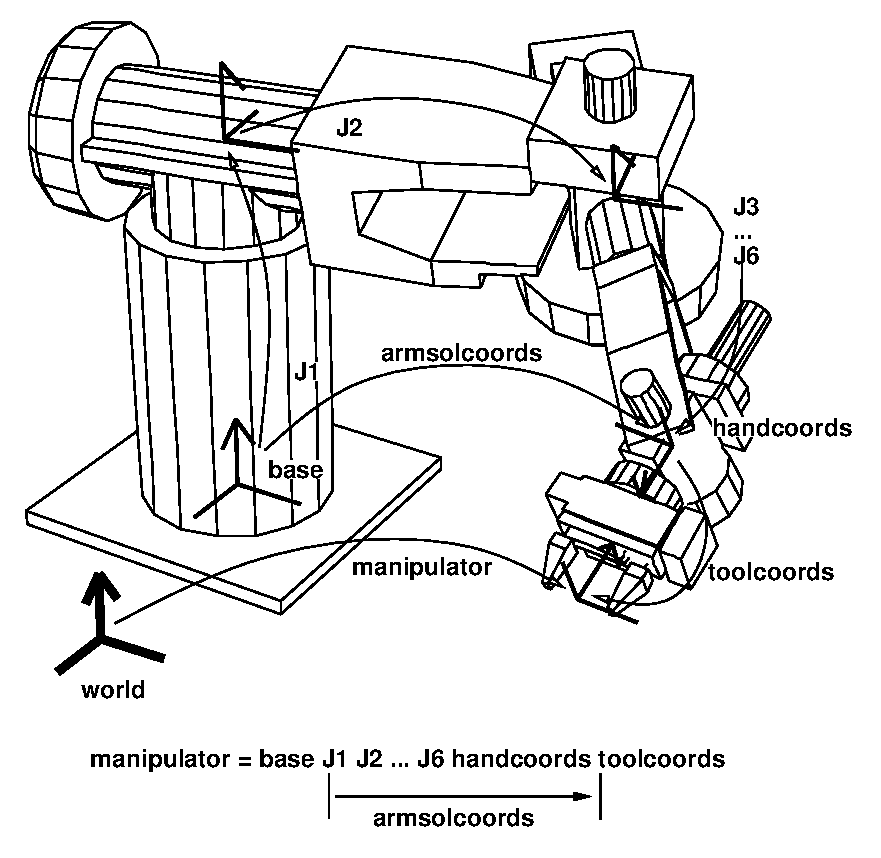
\includegraphics[height=100mm]{fig/eta3coords.ps}
%\epsfile{file=fig/eta3coords.ps,height=100mm}
\end{center}
\caption{\label{JointCoords}
relation between coordinate systems in a manipulator}

\end{figure}


各関節は、Brepで表現された幾何モデルを保持している。しかし、頂点の座標、
平面の方程式は常に現状を反映しているとは限らない。マニピュレータに対する
移動、回転などのメッセージでは座標系の更新だけを行い、頂点の座標は変化し
ない。これは、移動、回転が複数回続けて起こった場合の計算量を減らすためで
ある。更新は、マニピュレータに{\bf :worldcoords}メッセージを送る
ことで引き起こされる。


マニピュレータは、手先座標系で動作を指定することを主な目的としている。
関節角による指定には {\bf :config} を用いる。
引き数には6要素の列を与える。

\begin{verbatim}
  (send eta3 :config (float-vector pi/2 pi/2 0 1 0 1))
\end{verbatim}

{\bf :config}は、各関節角度が可動範囲に収まっていることを検査した後、
それらを回転させる。
この結果、マニピュレータの管理している座標系と
関節角度から定まる実際の手先の位置姿勢とが一致しなくなる。
両者を一致させるためには、{\bf :set-coords}メッセージを送る。
{\bf :set-coords}は、関節角度から順方向のキネマティクスを計算し、
最終的な手先座標系に対してさらにアーム解を解く。


例 ETA3のモデル生成とその描画
\begin{verbatim}
EusLisp 7.27 with Xlib created on Thu Sep 17 14:33:30 1992
(load "view.l")                                ;ウィンドウを開く
(load "/usr/local/eus/robot/eta3/eta3build.l") ;ETA3のモデルを生成する
(send *viewing* :look #f(2000 2000 2000))      ;視点を変える
(send-all (eta3arm-components eta3) :color 1)  ;物体の線の色を黒に変える
(send eta3 :config (float-vector 0 (/ -Pi 4.0) Pi/2 0 (/ -Pi 4.0) 0 ))
					       ;ETA3を関節角度の指定で動かす
(send eta3 :set-coords)                        ;上記参照
(draw eta3)                                    ;ETA3を描画する
\end{verbatim}

\newpage
